\PassOptionsToPackage{unicode=true}{hyperref} % options for packages loaded elsewhere
\PassOptionsToPackage{hyphens}{url}
\PassOptionsToPackage{dvipsnames,svgnames*,x11names*}{xcolor}
%
\documentclass[12pt,]{krantz}
\usepackage{lmodern}
\usepackage{amssymb,amsmath}
\usepackage{ifxetex,ifluatex}
\usepackage{fixltx2e} % provides \textsubscript
\ifnum 0\ifxetex 1\fi\ifluatex 1\fi=0 % if pdftex
  \usepackage[T1]{fontenc}
  \usepackage[utf8]{inputenc}
  \usepackage{textcomp} % provides euro and other symbols
\else % if luatex or xelatex
  \usepackage{unicode-math}
  \defaultfontfeatures{Ligatures=TeX,Scale=MatchLowercase}
    \setmonofont[Mapping=tex-ansi,Scale=0.7]{Source Code Pro}
\fi
% use upquote if available, for straight quotes in verbatim environments
\IfFileExists{upquote.sty}{\usepackage{upquote}}{}
% use microtype if available
\IfFileExists{microtype.sty}{%
\usepackage[]{microtype}
\UseMicrotypeSet[protrusion]{basicmath} % disable protrusion for tt fonts
}{}
\IfFileExists{parskip.sty}{%
\usepackage{parskip}
}{% else
\setlength{\parindent}{0pt}
\setlength{\parskip}{6pt plus 2pt minus 1pt}
}
\usepackage{xcolor}
\usepackage{hyperref}
\hypersetup{
            pdftitle={The Pueblo Farming Project},
            colorlinks=true,
            linkcolor=Maroon,
            citecolor=Blue,
            urlcolor=Blue,
            breaklinks=true}
\urlstyle{same}  % don't use monospace font for urls
\usepackage{longtable,booktabs}
% Fix footnotes in tables (requires footnote package)
\IfFileExists{footnote.sty}{\usepackage{footnote}\makesavenoteenv{longtable}}{}
\usepackage{graphicx,grffile}
\makeatletter
\def\maxwidth{\ifdim\Gin@nat@width>\linewidth\linewidth\else\Gin@nat@width\fi}
\def\maxheight{\ifdim\Gin@nat@height>\textheight\textheight\else\Gin@nat@height\fi}
\makeatother
% Scale images if necessary, so that they will not overflow the page
% margins by default, and it is still possible to overwrite the defaults
% using explicit options in \includegraphics[width, height, ...]{}
\setkeys{Gin}{width=\maxwidth,height=\maxheight,keepaspectratio}
\setlength{\emergencystretch}{3em}  % prevent overfull lines
\providecommand{\tightlist}{%
  \setlength{\itemsep}{0pt}\setlength{\parskip}{0pt}}
\setcounter{secnumdepth}{5}
% Redefines (sub)paragraphs to behave more like sections
\ifx\paragraph\undefined\else
\let\oldparagraph\paragraph
\renewcommand{\paragraph}[1]{\oldparagraph{#1}\mbox{}}
\fi
\ifx\subparagraph\undefined\else
\let\oldsubparagraph\subparagraph
\renewcommand{\subparagraph}[1]{\oldsubparagraph{#1}\mbox{}}
\fi

% set default figure placement to htbp
\makeatletter
\def\fps@figure{htbp}
\makeatother

\usepackage{booktabs}
\usepackage{longtable}
\usepackage[bf,singlelinecheck=off]{caption}

\setmainfont[UprightFeatures={SmallCapsFont=AlegreyaSC-Regular}]{Alegreya}

\usepackage{framed,color}
\definecolor{shadecolor}{RGB}{248,248,248}

\renewcommand{\textfraction}{0.05}
\renewcommand{\topfraction}{0.8}
\renewcommand{\bottomfraction}{0.8}
\renewcommand{\floatpagefraction}{0.75}

\renewenvironment{quote}{\begin{VF}}{\end{VF}}
\let\oldhref\href
\renewcommand{\href}[2]{#2\footnote{\url{#1}}}

\ifxetex
  \usepackage{letltxmacro}
  \setlength{\XeTeXLinkMargin}{1pt}
  \LetLtxMacro\SavedIncludeGraphics\includegraphics
  \def\includegraphics#1#{% #1 catches optional stuff (star/opt. arg.)
    \IncludeGraphicsAux{#1}%
  }%
  \newcommand*{\IncludeGraphicsAux}[2]{%
    \XeTeXLinkBox{%
      \SavedIncludeGraphics#1{#2}%
    }%
  }%
\fi

\makeatletter
\newenvironment{kframe}{%
\medskip{}
\setlength{\fboxsep}{.8em}
 \def\at@end@of@kframe{}%
 \ifinner\ifhmode%
  \def\at@end@of@kframe{\end{minipage}}%
  \begin{minipage}{\columnwidth}%
 \fi\fi%
 \def\FrameCommand##1{\hskip\@totalleftmargin \hskip-\fboxsep
 \colorbox{shadecolor}{##1}\hskip-\fboxsep
     % There is no \\@totalrightmargin, so:
     \hskip-\linewidth \hskip-\@totalleftmargin \hskip\columnwidth}%
 \MakeFramed {\advance\hsize-\width
   \@totalleftmargin\z@ \linewidth\hsize
   \@setminipage}}%
 {\par\unskip\endMakeFramed%
 \at@end@of@kframe}
\makeatother

\newenvironment{Shaded}{\begin{kframe}}{\end{kframe}}

\newenvironment{rmdblock}[1]
  {
  \begin{itemize}
  \renewcommand{\labelitemi}{
    \raisebox{-.7\height}[0pt][0pt]{
      {\setkeys{Gin}{width=3em,keepaspectratio}\includegraphics{images/#1}}
    }
  }
  \setlength{\fboxsep}{1em}
  \begin{kframe}
  \item
  }
  {
  \end{kframe}
  \end{itemize}
  }
\newenvironment{rmdnote}
  {\begin{rmdblock}{note}}
  {\end{rmdblock}}
\newenvironment{rmdcaution}
  {\begin{rmdblock}{caution}}
  {\end{rmdblock}}
\newenvironment{rmdimportant}
  {\begin{rmdblock}{important}}
  {\end{rmdblock}}
\newenvironment{rmdtip}
  {\begin{rmdblock}{tip}}
  {\end{rmdblock}}
\newenvironment{rmdwarning}
  {\begin{rmdblock}{warning}}
  {\end{rmdblock}}

\usepackage{makeidx}
\makeindex

\urlstyle{tt}

\usepackage{amsthm}
\makeatletter
\def\thm@space@setup{%
  \thm@preskip=8pt plus 2pt minus 4pt
  \thm@postskip=\thm@preskip
}
\makeatother

\frontmatter
\usepackage[]{natbib}
\bibliographystyle{apalike}

\title{The Pueblo Farming Project}
\providecommand{\subtitle}[1]{}
\subtitle{A collaboration between Hopi Farmers and\\
the Crow Canyon Archaeological Center}
\author{Paul Ermigiotti,\\
Mark Varien,\\
Erin Bohm,\\
Kyle Bocinsky, and\\
the Hopi Cultural Resources Advisory Team}
\date{2017-11-29}

\let\BeginKnitrBlock\begin \let\EndKnitrBlock\end
\begin{document}
\maketitle

%\cleardoublepage\newpage\thispagestyle{empty}\null
%\cleardoublepage\newpage\thispagestyle{empty}\null
%\cleardoublepage\newpage
%	\thispagestyle{empty}
%	\begin{center}
%	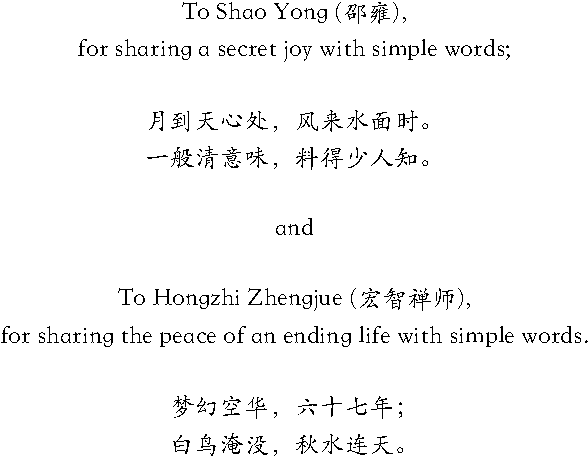
\includegraphics{images/dedication.pdf}
%	\end{center}
%
%\setlength{\abovedisplayskip}{-5pt}
%\setlength{\abovedisplayshortskip}{-5pt}

{
\hypersetup{linkcolor=}
\setcounter{tocdepth}{2}
\tableofcontents
}
\listoftables
\listoffigures
\hypertarget{preface}{%
\chapter*{Preface}\label{preface}}


The Pueblo Farming Project, or PFP, is an ongoing collaboration between
the Hopi tribe and the Crow Canyon Archaeological Center. The PFP
examines traditional Pueblo Indian farming techniques to help us
understand ancient farming in the Mesa Verde region of southwestern
Colorado. The project conducts research, develops educational programs,
and pursues Hopi interests in corn and corn farming as an essential
element of their culture. This e-book presents the methods and results
from the Pueblo Farming Project, as well as a set of lesson plans
developed for middle school students to learn about Hopi agriculture.


\includegraphics{images/by-nc-sa.png}\\
The online version of this book is licensed under the
\href{http://creativecommons.org/licenses/by-nc-sa/4.0/}{Creative
Commons Attribution-NonCommercial-ShareAlike 4.0 International License}.

\hypertarget{how-to-use-this-book}{%
\section*{How to use this book}\label{how-to-use-this-book}}


\hypertarget{saving-and-printing}{%
\section*{Saving and printing}\label{saving-and-printing}}


\hypertarget{comments-and-feedback}{%
\section*{Comments and feedback}\label{comments-and-feedback}}


\hypertarget{acknowledgments}{%
\section*{Acknowledgments}\label{acknowledgments}}


\BeginKnitrBlock{flushright}
Paul Ermigiotti, Mark Varien, Erin Bohm, and Kyle Bocinsky Cortez,
Colorado
\EndKnitrBlock{flushright}

\mainmatter

\hypertarget{introduction}{%
\chapter{Introduction}\label{introduction}}

\hypertarget{what-was-the-pfp}{%
\section{What was the PFP?}\label{what-was-the-pfp}}

\hypertarget{history}{%
\subsection*{History}\label{history}}


\hypertarget{research-goals}{%
\subsection*{Research goals}\label{research-goals}}


\hypertarget{hopi-interests}{%
\subsection*{Hopi interests}\label{hopi-interests}}


\hypertarget{educational-products}{%
\subsection*{Educational products}\label{educational-products}}


Highlight MSTFP

\hypertarget{who-were-the-participants}{%
\section{Who were the participants?}\label{who-were-the-participants}}

\hypertarget{where-did-it-take-place}{%
\section{Where did it take place?}\label{where-did-it-take-place}}

\hypertarget{when-did-it-take-place}{%
\section{When did it take place?}\label{when-did-it-take-place}}

\hypertarget{who-funded-the-pfp}{%
\section{Who funded the PFP?}\label{who-funded-the-pfp}}

\hypertarget{the-story-of-maize}{%
\chapter{The Story of Maize}\label{the-story-of-maize}}

\hypertarget{origins}{%
\section{Origins}\label{origins}}

\hypertarget{the-people-of-corn}{%
\section{The people of corn}\label{the-people-of-corn}}

\hypertarget{a-world-of-corn}{%
\section{A world of corn}\label{a-world-of-corn}}

\hypertarget{the-life-cycle-of-maize}{%
\chapter{The life-cycle of maize}\label{the-life-cycle-of-maize}}

\hypertarget{what-maize-needs-to-flourish}{%
\chapter{What maize needs to
flourish}\label{what-maize-needs-to-flourish}}

\hypertarget{soil}{%
\section{Soil}\label{soil}}

\hypertarget{water}{%
\section{Water}\label{water}}

\hypertarget{heat-and-sunlight}{%
\section{Heat and sunlight}\label{heat-and-sunlight}}

\hypertarget{gdd-sidebar}{%
\subsection*{GDD sidebar}\label{gdd-sidebar}}


\hypertarget{the-pfp-field-experiments}{%
\chapter{The PFP Field Experiments}\label{the-pfp-field-experiments}}

\hypertarget{procedure}{%
\section{Procedure}\label{procedure}}

\hypertarget{the-pfp-environment}{%
\section{The PFP environment}\label{the-pfp-environment}}

\hypertarget{soils-in-the-gardens}{%
\subsection*{Soils in the gardens}\label{soils-in-the-gardens}}


\hypertarget{cortez-weather-and-ccac-weather-stations}{%
\subsection{Cortez weather and CCAC weather
stations}\label{cortez-weather-and-ccac-weather-stations}}

\hypertarget{precipitation}{%
\subsubsection{Precipitation}\label{precipitation}}

\hypertarget{temperature}{%
\subsubsection{Temperature}\label{temperature}}

\hypertarget{gdd}{%
\subsubsection{GDD}\label{gdd}}

\hypertarget{results}{%
\section{Results}\label{results}}

\hypertarget{maize-growth-analysis}{%
\subsection*{Maize growth analysis}\label{maize-growth-analysis}}


\hypertarget{maize-production}{%
\subsection*{Maize production}\label{maize-production}}


\hypertarget{ear-diversity}{%
\subsubsection{Ear diversity}\label{ear-diversity}}

\hypertarget{yields-through-time}{%
\subsubsection{Yields through time}\label{yields-through-time}}

\hypertarget{maize-genetics}{%
\subsection*{Maize genetics}\label{maize-genetics}}


\hypertarget{what-we-learned}{%
\chapter{What we learned}\label{what-we-learned}}

\hypertarget{the-resilience-of-hopi-corn}{%
\section{The resilience of Hopi
corn}\label{the-resilience-of-hopi-corn}}

\hypertarget{improving-our-understanding-of-mesa-verde-history}{%
\section{Improving our understanding of Mesa Verde
history}\label{improving-our-understanding-of-mesa-verde-history}}

\hypertarget{culture-matters}{%
\section{Culture matters!}\label{culture-matters}}

\hypertarget{lesson-plans-for-educators}{%
\chapter{Lesson plans for educators}\label{lesson-plans-for-educators}}

\hypertarget{the-people-of-corn-1}{%
\section{The People of Corn}\label{the-people-of-corn-1}}

\hypertarget{farming-through-drought}{%
\section{Farming Through Drought}\label{farming-through-drought}}

\hypertarget{know-your-soil}{%
\section{Know Your Soil}\label{know-your-soil}}

\hypertarget{ancient-technologies}{%
\section{Ancient Technologies}\label{ancient-technologies}}

\hypertarget{the-short-blue-ear}{%
\section{The Short Blue Ear}\label{the-short-blue-ear}}

\hypertarget{references}{%
\chapter*{References}\label{references}}


\bibliography{book.bib,packages.bib}

\backmatter
\printindex

\end{document}
